\documentclass[11pt]{article}
\usepackage{a4,fancyhdr,moreverb,epsfig,amssymb,amsmath,ifthen}
\usepackage[utf8]{inputenc}
\usepackage[english]{babel}
\usepackage{mathtools}
\usepackage{lstautogobble}
\usepackage[framed,numbered]{mcode}
\usepackage{listings}
\usepackage{subcaption}
\usepackage{amsthm}
\textwidth 455pt \oddsidemargin 0mm
\parindent 12pt
\textheight 685pt % old : 665pt
\textheight 697pt
\topmargin -40pt  % old -70pt
\newcommand{\cpp}{C\raisebox{.4ex}{\tiny ++}}
\renewcommand{\vec}{\underline}
\newcommand{\va}{\underline{a}}
\newcommand{\vb}{\underline{b}}
\newcommand{\vc}{\underline{c}}
\newcommand{\vh}{\underline{h}}
\newcommand{\ve}{\underline{e}}
\newcommand{\vg}{\underline{g}}
\newcommand{\vp}{\underline{p}}
\newcommand{\vq}{\underline{q}}
\newcommand{\vu}{\underline{u}}
\newcommand{\vv}{\underline{v}}
\newcommand{\vw}{\underline{w}}
\newcommand{\vx}{\underline{x}}
\newcommand{\vy}{\underline{y}}
\newcommand{\vz}{\underline{z}}
\newcommand\myeq{\stackrel{\mathclap{\normalfont\mbox{cgs}}}{=}}
\newcommand{\dd}[1]{\mathrm{d}#1}


\usepackage{graphicx}
\graphicspath{ {./images/} }

\lstset{
   basicstyle=\fontsize{9}{11}\selectfont\ttfamily
}
\begin{document}
\pagestyle{fancyplain}
\lhead{\fancyplain{}{\sf M4S18B2 Machine Learning}}
\rhead{\fancyplain{}{\sf Omar Haque}}
\cfoot{}{}
\begin{center} \Large
Machine Learning - Coursework 1 \\[4mm]
\end{center}
\textbf{Calculate and plot the average face of the training set, then write a function to find a PCA basis of size M, where the inputs will be M and X, the matrix containing the training set. Clearly describe all aspects of your function, then use it to plot the first 5 eigenfaces of the training set.}


To calculate the average face of the training set, I simply calculate the average pixel values for each pixel across the trainings set.
\begin{lstlisting}[linewidth=18.4cm,language=R]
library(rARPACK)
library(philentropy)
# I load the raw csv's
faces.train.inputs <- read.csv("./2018_ML_Assessed_Coursework_1_Data/
                               Faces_Train_Inputs.csv",head=FALSE)
faces.train.label <- read.csv("./2018_ML_Assessed_Coursework_1_Data/
                              Faces_Train_Labels.csv",head=FALSE)
faces.test.inputs <- read.csv("./2018_ML_Assessed_Coursework_1_Data/
                              Faces_Test_Inputs.csv",head=FALSE)
faces.test.label <- read.csv("./2018_ML_Assessed_Coursework_1_Data/
                             Faces_Test_Labels.csv",head=FALSE)
# I turn the input values into a list of 320 matrices, each matrix a 112 x 92 value 
# of pixels corresponding to each image .. I need to use lapply again on the 
#result because apply gives the matrices in a weird form
faces.train.inputs.cleaned <- lapply(apply(X=faces.train.inputs, 
                                           MARGIN=1, 
                                           function(x) list(matrix(as.numeric(x), 
                                           nrow = 112))), "[[", 1)
# Here I calculate the average face
avg.face <- Reduce('+', faces.train.inputs.cleaned) / 
  length(faces.train.inputs.cleaned)
image(avg.face)
\end{lstlisting}
Please see figure 1 for results. \\

\begin{figure}[b]
\caption{Average face of the training set}
\centering
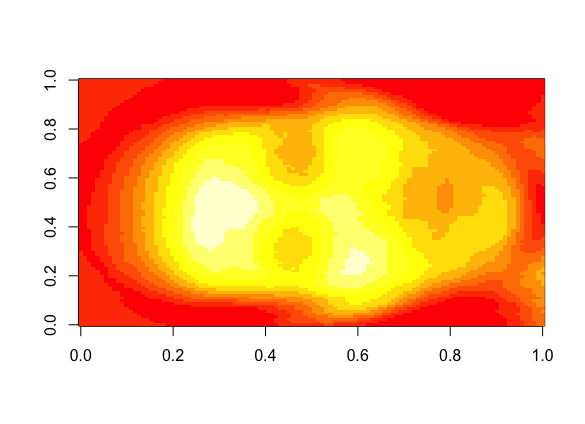
\includegraphics[width=0.5\textwidth]{average}
\end{figure}

The following function returns the PCA basis of size M as specified. I added a default parameter which also allows access to the eigenvalues associated with each vector of the eigenbasis.

The function works exactly as the PCA described in lectures. Calculate the centralised data matrix, $X$, and then calculate the first M eigenvectors for the covariance matrix $\frac{XX^{T}}{n}$.

\begin{lstlisting}[linewidth=18.4cm,language=R]
find.pca.basis <- function(M,X, return.full.results = FALSE){
  n <- dim(X)[1] # The number of images
  # Turn the input data into a matrix and transpose it
  X.data.matrix <- data.matrix(t(X))
  # Centralise the data matrix
  means <- rowMeans(X.data.matrix) # calculate row means
  data.matrix.centralised <- X.data.matrix - means %*% t(rep(1,n)) # and subtract
  # Calculate the covariance matrix as defined in lectures
  covariance.matrix <- (data.matrix.centralised %*% t(data.matrix.centralised)) / n
  # Now I need to compute the first M eigenvectors/ eigenvalues using the 
  # R package rARPACK
  results <- eigs_sym(covariance.matrix,k=M,which="LM")
  if (return.full.results){
    return(results)
  } else{
    return(results$vectors)
  }
}
\end{lstlisting}

The code below then plots the first 5 eigenfaces of the training set. This means simply calculating the eigenbasis for M = 5, and then plotting the vectors in the resulting eigenbasis.
\begin{lstlisting}[linewidth=18.4cm,language=R]
eigenbasis <- find.pca.basis(5,faces.train.inputs)
par(mfrow=c(2,3))
for (i in 1:5){
  # eigenbasis[,i] corresponds to the i'th eigenvector.
  image(matrix(eigenbasis[,i], nrow = 112),useRaster=TRUE, axes=FALSE,main=i)
}
par(mfrow=c(1,1))
\end{lstlisting}

The results can be seen in figure 2.

\begin{figure}
\caption{First 5 Eigenfaces of the  training set}
\centering
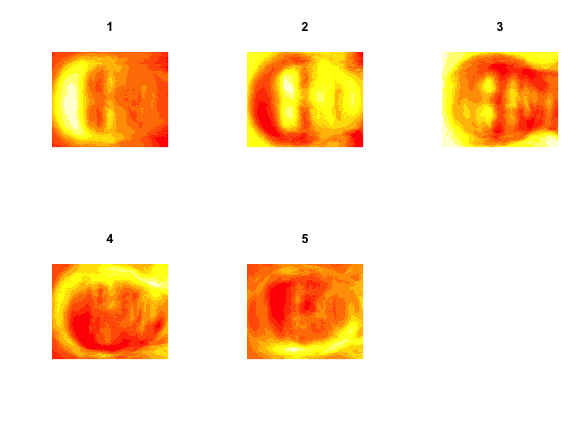
\includegraphics[width=0.8\textwidth]{eigenface}
\end{figure}


\begin{itemize}
\item \textbf{Choose a single face and project it into a PCA basis for dimension M = 5, 10, 50, then plot the results.}
\end{itemize}

Here is the code to project the first image of the training set onto the PCA basis for dimensions 5,10 and 50.
\begin{lstlisting}[linewidth=18.4cm,language=R]
# initialise the dimensions and face used.
dimensions <- c(5,10,50)
single.face <- 1
means <- as.vector(avg.face) # convert the mean face back into a vector

# iterate through the dimensions considered
for (i in dimensions){
  
  # compute the eigenbasis using the function created
  eigenbasis <- find.pca.basis(i,faces.train.inputs)
  # calculate the projection values in this pca basis
  projection.vals <- t(as.numeric(faces.train.inputs[single.face,]) - 
                         means) %*% eigenbasis
  # calculate the actual face in this basis
  projection.vector <- eigenbasis %*% as.numeric(as.list(projection.vals))
  
  # carry out the plot
  image(matrix(projection.vector, nrow = 112),useRaster=TRUE, 
        axes=FALSE,main=paste("dimension",i,sep=" "))
}

# and here's the original image
image(matrix(as.numeric(faces.train.inputs[single.face,]), nrow = 112), 
      useRaster=TRUE, axes=FALSE, main="Original Image")
\end{lstlisting}
Please see Figure 3 for the results of this code.


    \begin{figure}[t!]
        \caption[ The average and standard deviation of critical parameters ]
	{\small The projection of training image 1 onto PCA bases of different dimensions} 
        \centering
        
        \begin{subfigure}[b]{0.375\textwidth}
            \centering
            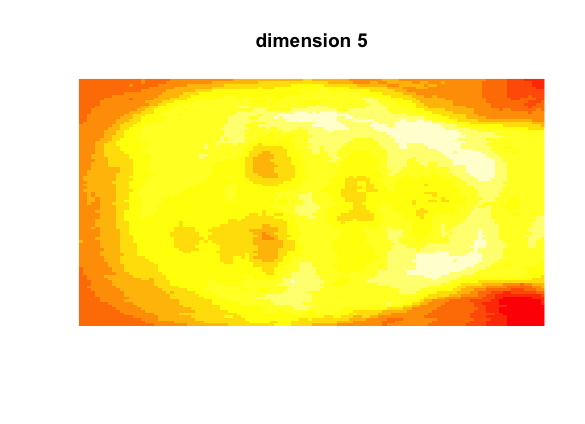
\includegraphics[width=\textwidth]{5}
            \caption[Dimension 5]%

            \label{fig:mean and std of net14}
        \end{subfigure}
        \hfill
        \begin{subfigure}[b]{0.375\textwidth}  
            \centering 
            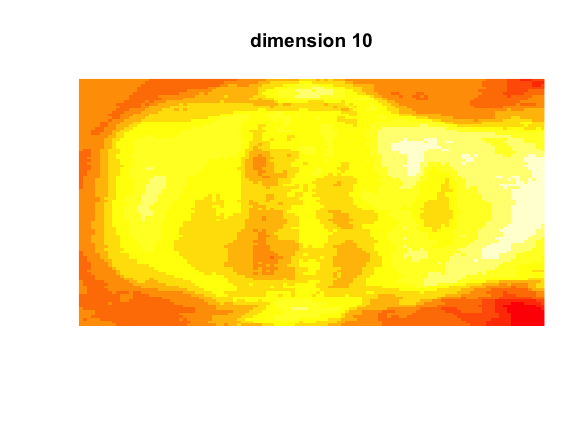
\includegraphics[width=\textwidth]{10}
            \caption[]%

            \label{fig:mean and std of net24}
        \end{subfigure}
        \vskip\baselineskip
        \begin{subfigure}[b]{0.375\textwidth}   
            \centering 
            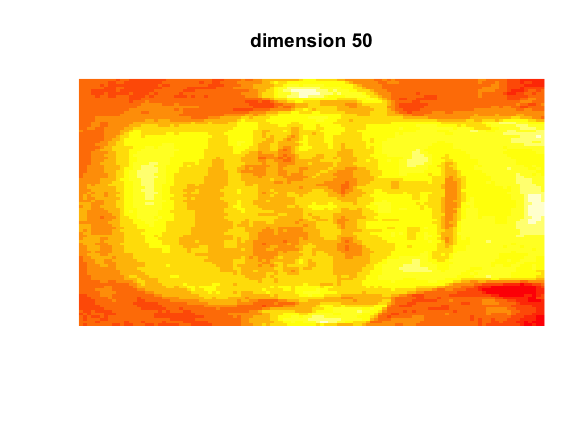
\includegraphics[width=\textwidth]{50}
            \caption[]%

            \label{fig:mean and std of net34}
        \end{subfigure}
        \quad
        \begin{subfigure}[b]{0.375\textwidth}   
            \centering 
            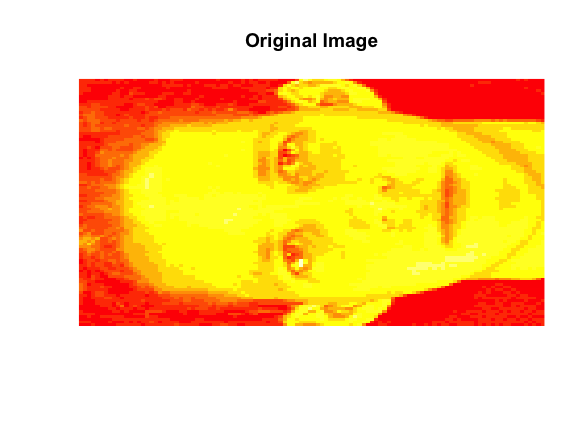
\includegraphics[width=\textwidth]{orig}
            \caption[]%
 
            \label{fig:mean and std of net44}
        \end{subfigure}


        \label{fig:mean and std of nets}
    \end{figure}

\begin{itemize}
\item \textbf{Plot a graph of the mean squared error of each lower dimensional approximation of this chosen face, with the dimensionality plotted along the x-axis. Is there a clear point at which we can choose a good approximation? Discuss how we should choose the appropriate dimensionality of the approximation.}
\end{itemize}
\textbf{setup:}
We can derive a nice form for the mean square error. Let $X$ be our \textbf{centralised} data matrix with $n$ observations of $p$ variables. Consider PCA of $k$ dimensions. Let $\hat{X}$ be the projection of $X$ onto this basis of dimension $k$. Denote the i'th eigenvector of the covariance matrix of $X$ by $Y_{i}$. \\
\textbf{form of MSE:}
Now we have $E[||X||^{2}] = \Sigma_{i=1}^{n} Var(X_{i})$. From the spectral decomposition of the covariance matrix we have that $\Sigma_{i=1}^{n} Var(X_{i}) = \Sigma_{i=1}^{n} \lambda_{i}$, where the $\lambda_{i}$ correspond to the eigenvalues of the covariance matrix we calculate during the PCA algorithm. Then we have that the $MSE := E[||X - \hat{X}  ||^{2}] = \Sigma_{i=1}^{n} \lambda_{i} - \Sigma_{i=1}^{k} Var(Y_{i}) =  \Sigma_{i=1}^{n} \lambda_{i} - \Sigma_{i=1}^{k} \lambda_{i} = \Sigma_{i=k+1}^{n} \lambda_{i}$

We approximate the true total variance here by the sum of the first 320 eigenvalues. Please see figure 4 for the results of this code. 

\begin{lstlisting}[linewidth=18.4cm,language=R]
# First I calculate the full pca basis (and all the assosciated eigenvalues)
full.results <- find.pca.basis(320,faces.train.inputs,return.full.results = TRUE)

# the mean square error is equal to the total variance minus the sum of the 
# eigenvalues for components not used 
mses <- (cumsum(full.results$values)[length(full.results$values)] - 
           cumsum(full.results$values) )
plot(mses,xlab="Dimensionality of PCA",ylab="Mean Square Error")
\end{lstlisting}


From the graph in figure 4, we see that the mean square error rapidly decreases in linear steps of dimensionality up to around $k = 50$. After this point, the rate of decay is slower and it suggests that taking further dimensions does not improve the mean square error at the same rate. This "elbow point" of 50 is where we should choose our appropriate dimension. KNN scales well for our problem however, so I will use the less strict cutoff of k = 100.


\begin{figure}[t!]
\caption{Mean Squared Error as a function of PCA dimension}
\centering
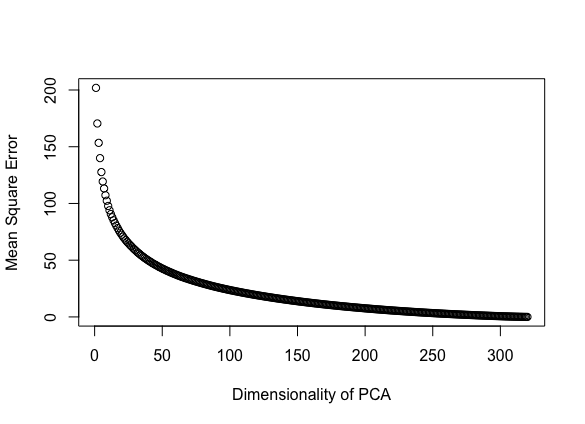
\includegraphics[width=0.6\textwidth]{mse}
\end{figure}
\begin{itemize}
\item \textbf{Write a function implementing a K-nearest neighbour classifier and investigate its use on the face recognition dataset. Make some recommendations regarding how to best set up this algorithm for this particular application.}
\end{itemize}
Here is the code for my K-nearest neighbour classifier 
\begin{lstlisting}[linewidth=18.4cm,language=R]
k.nearest.neighbours <- function(training.data.matrix, training.data.labels, 
                                 testing.data.matrix,K = 4, 
                                 distance.type = "squared_euclidean"){
  # Make sure all the data is numeric
  training.data.matrix <- data.matrix(training.data.matrix)
  testing.data.matrix <- data.matrix(testing.data.matrix)
  training.data.labels <- as.numeric(training.data.labels)
  # Initialise the list which will take the classifications
  classifiers <- c()
  # iterate through every row of the testing matrix
  for (i in 1:dim(testing.data.matrix)[1]){
    # compute the distance of this row of the testing matrix to every other 
    # row in the training set
    all.distances <- apply(training.data.matrix, MARGIN=1, 
                           function(x) distance(rbind(testing.data.matrix[i,],x), 
                                                method=distance.type))
    # sort these distances in increasing order.
    sorted.distances <- sort(all.distances,index.return=TRUE)
    
    # Look at the k closest rows in the training set to this testing row. 
    # Whichever classification comes up the most - is the classification we 
    # will give this particular row.
    all.counts <- tabulate(training.data.labels[sorted.distances$ix[1:K]])
    sorted.counts <- sort(all.counts, index.return=TRUE, decreasing=TRUE)
    ## these are all the voters which share the maximum score
    max.votes <- which(sorted.counts$x == sorted.counts$x[1])
    if (length(max.votes) > 1){
      # if it's a split vote, randomly select one.
      voter <- sample(1:length(max.votes),size=1)
    } else {
      # else, there's only one.
      voter <- 1
    }
    # set the classification.
    classification <- sorted.counts$ix[voter]
    classifiers <- c(classifiers,classification)

  }
  
  return(classifiers)
  
}
\end{lstlisting}

First I perform PCA on the data to transform all the images onto the basis given by the training data, for k = 100. Then I computed the accuracy using 3 distance functions: Manhattan, Euclidean and Sorensen. The accuracy of the 3 appraoches varies as follows:
\begin{lstlisting}[linewidth=18.4cm,language=R]
## TRY pca preprocessing
## compute the eigenbasis then move all of the data into this PCA space
eigenbasis <- find.pca.basis(100,faces.train.inputs)
faces.train.new.basis <- lapply(X = c(1:320),
                                FUN=function(x) t(as.numeric(faces.train.inputs[x,]) 
                                                  - means) %*% eigenbasis)
faces.train.new.basis <- do.call("rbind",faces.train.new.basis)
faces.test.new.basis <- lapply(X = c(1:80),
                               FUN=function(x) t(as.numeric(faces.test.inputs[x,]) -
                                                   means) %*% eigenbasis)
faces.test.new.basis <- do.call("rbind",faces.test.new.basis)
# initialise the list of accuracies
accuracy.sor.list <- c()
accuracy.man.list <- c()
accuracy.sq.list <- c()
for (i in 1:8){ # these are the values of k we will use
  # calculate the classes for each distance type
  classes.sor <- k.nearest.neighbours(training.data.matrix = faces.train.new.basis , 
                                      training.data.labels = faces.train.label, 
                                      testing.data.matrix = faces.test.new.basis,K=i, 
                                      distance.type = "sorensen")
  classes.man <- k.nearest.neighbours(training.data.matrix = faces.train.new.basis, 
                                      training.data.labels = faces.train.label, 
                                      testing.data.matrix = faces.test.new.basis,K=i,
                                      distance.type = "manhattan")
  classes.sq <- k.nearest.neighbours(training.data.matrix = faces.train.new.basis, 
                                       training.data.labels = faces.train.label, 
                                      testing.data.matrix = faces.test.new.basis,K=i, 
                                       distance.type = "squared_euclidean")
  classes.actual <- as.integer(faces.test.label)
  ## add the accuracy to the list of accuracies..
  accuracy.sor <- 100*length(which(classes.sor == classes.actual)) / 
    length(classes.actual)
  accuracy.sor.list <- c(accuracy.sor.list,accuracy.sor)
  accuracy.man <- 100*length(which(classes.man == classes.actual)) / 
    length(classes.actual)
  accuracy.man.list <- c(accuracy.man.list,accuracy.man)
  accuracy.sq <- 100*length(which(classes.sq == classes.actual)) / 
    length(classes.actual)
  accuracy.sq.list <- c(accuracy.sq.list,accuracy.sq)
}

## now check and plot them
# plot all three on same graph
fullmat <- cbind(sorensen=accuracy.sor.list,manhattan=accuracy.man.list,
                 euclidean=accuracy.sq.list)
matplot(fullmat, type = c("b"),pch=1,col = 1:3,ylab="accuracy",xlab="k") #plot
legend("right", legend = colnames(fullmat), col=1:3, pch=1) 
\end{lstlisting}

The results can be seen in figure 5 below. The regular Euclidean norm tended to perform best over varying values of k. In this particular training/test split, the absolute best accuracy was found with K = 1 for the euclidean norm with 96.25\% accuracy. This is incredibly high considering we have broken the problem down from 10304 dimensions to 100.

\begin{figure}[b!]
\caption{PCA preprocessing for KNN accuracy}
\centering
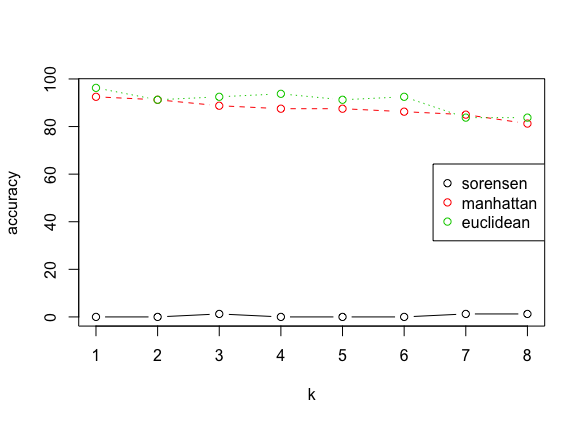
\includegraphics[width=0.6\textwidth]{final}
\end{figure}

\end{document}
